\documentclass{article}
\usepackage{graphicx} % Required for inserting images
\usepackage{tikz}

\title{TikZ Freeform Annotation}
\author{elerac}
\date{}

\begin{document}

\maketitle

\section{Showcase}

\begin{figure}[tbh]
    \centering
    \begin{minipage}{0.5\hsize}
        \centering
        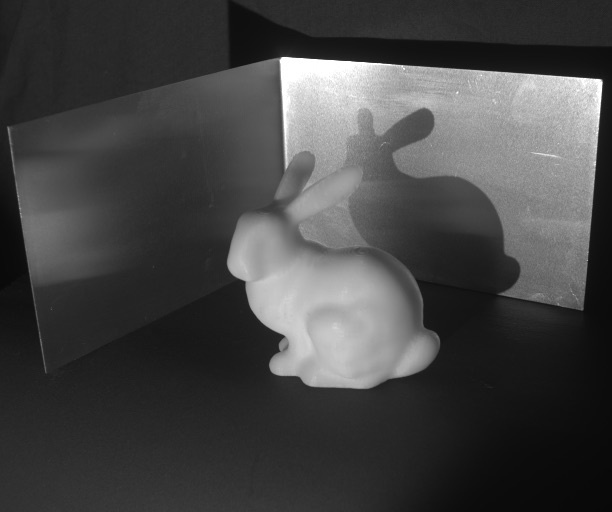
\includegraphics[width=0.98\hsize]{figures/bunny.jpg}
        (a) Standard includegraphics
    \end{minipage}%
    \begin{minipage}{0.5\hsize}
        \centering
        \scalebox{0.98}{
            \begin{tikzpicture}[x=\linewidth/612.0, y=-\linewidth/612.0, transform shape, scale=1.0]
    \node[inner sep=0] (image) at (0,0) {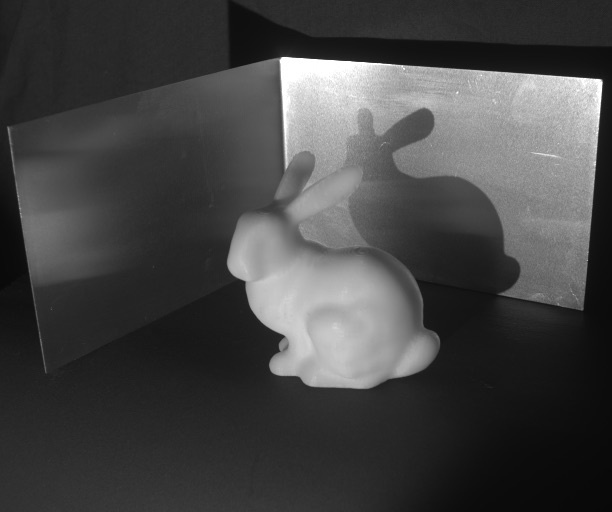
\includegraphics[width=\hsize]{figures/bunny.jpg}};
    \begin{scope}[shift={(image.north west)}]
        \draw[red] ++(303, 151) -- ++(7, 0) .. controls (313.6, 156.2) and (315.2, 158) .. ++(5, 17) .. controls (310.9, 173.2) and (306.7, 182.1) .. ++(-10, 21) -- ++(3, 0) .. controls (312.5, 182.3) and (333.7, 171) .. ++(34, -21) -- ++(19, 0) -- ++(1, 3) .. controls (366.2, 178.2) and (357.5, 188.5) .. ++(-8, 21) .. controls (349.6, 196.5) and (344.4, 202.6) .. ++(-16, 13) .. controls (333.8, 206.6) and (330.7, 205.2) .. ++(-11, 2) .. controls (316.9, 212) and (307, 219.7) .. ++(-28, 20) .. controls (299.9, 231.9) and (302, 237.2) .. ++(7, 12) .. controls (309.3, 241.3) and (327.7, 248) .. ++(26, 10) .. controls (344.6, 252) and (364.3, 243.2) .. ++(47, -1) .. controls (400.3, 255) and (417.4, 276.2) .. ++(44, 51) -- ++(0, 27) .. controls (428.2, 329.2) and (438, 332.6) .. ++(17, 13) .. controls (445.3, 355.8) and (422.6, 371.2) .. ++(-27, 36) .. controls (405.6, 377.9) and (397.1, 376.2) .. ++(-24, 4) .. controls (382.8, 381.1) and (376.7, 387.2) .. ++(-19, 10) -- ++(-59, -2) .. controls (304.3, 385.1) and (302.5, 377.9) .. ++(-14, -11) .. controls (282.6, 370.9) and (271.5, 383.4) .. ++(-28, -12) .. controls (270.6, 362.1) and (270.5, 359.1) .. ++(3, -7) -- ++(7, -5) -- ++(1, 0) -- ++(-1, -8) .. controls (280.1, 340.6) and (283.1, 339.6) .. ++(5, -9) .. controls (267.3, 331.2) and (253, 317.5) .. ++(-36, -33) -- ++(-3, -20) .. controls (238.6, 276.5) and (229.8, 276.2) .. ++(-18, -15) .. controls (225.1, 260.9) and (228.9, 253.9) .. ++(3, -17) .. controls (233.5, 237.5) and (234.3, 217) .. ++(16, -37) .. controls (254.3, 207.5) and (267.6, 210.1) .. ++(27, -11) -- ++(3, -11) .. controls (279.5, 182.7) and (289.7, 158.8) .. ++(20, -37) .. controls (298, 152.5) and (301.1, 152.4) .. ++(7, -3) -- cycle; % cls-1
        \draw[green] ++(603, 80) -- ++(-20, 232) .. controls (577.9, 311.9) and (573, 310.2) .. ++(-14, -3) -- ++(-6, 0) .. controls (555.2, 306.6) and (544.8, 305.4) .. ++(-26, -6) -- ++(-6, 0) -- ++(0, -1) -- ++(-5, 0) -- ++(0, -1) -- ++(-6, 0) .. controls (503.6, 296) and (483.4, 295) .. ++(-53, -11) -- ++(-6, 0) .. controls (453.2, 287.6) and (442.8, 286.4) .. ++(-26, -6) -- ++(-6, 0) -- ++(0, -1) .. controls (425.3, 281.9) and (420.5, 283.3) .. ++(-11, -2) -- ++(-1, 0) -- ++(-1, -5) -- ++(-3, -2) -- ++(0, -2) -- ++(-2, -1) -- ++(0, -2) -- ++(-3, -2) -- ++(-6, -7) -- ++(-2, 0) -- ++(-3, -4) -- ++(-2, 0) -- ++(-1, -2) -- ++(-2, 0) -- ++(-2, -3) -- ++(-3, 0) -- ++(-1, -2) -- ++(-2, 0) -- ++(0, -1) -- ++(-4, -1) -- ++(0, -1) -- ++(-31, -1) -- ++(0, 1) -- ++(-17, 1) -- ++(0, -1) -- ++(-5, 0) -- ++(0, -1) -- ++(-6, -2) -- ++(0, -1) -- ++(-2, 0) -- ++(0, -1) -- ++(-14, -4) .. controls (303.7, 234.3) and (300.3, 229.4) .. ++(-3, -10) -- ++(0, -2) -- ++(3, -1) -- ++(3, -4) -- ++(5, -1) -- ++(2, -3) -- ++(2, 0) -- ++(1, -2) -- ++(3, 0) -- ++(1, -2) -- ++(4, -1) -- ++(1, -2) -- ++(3, 0) -- ++(0, -1) -- ++(6, -1) -- ++(1, 1) -- ++(0, -1) -- ++(3, -1) -- ++(1, -2) -- ++(6, -2) -- ++(5, -6) -- ++(2, 0) -- ++(2, -2) -- ++(0, -2) -- ++(4, -3) .. controls (362.9, 184.8) and (364.9, 177.8) .. ++(5, -18) -- ++(-1, 0) -- ++(0, -2) -- ++(-3, -2) -- ++(0, -1) -- ++(-20, 0) .. controls (338.1, 170.5) and (337.5, 167.2) .. ++(-8, 4) -- ++(-1, 2) -- ++(-3, 1) -- ++(0, 1) -- ++(-5, 1) -- ++(0, 1) -- ++(-2, 0) -- ++(-1, 2) -- ++(-4, 1) -- ++(-1, 2) -- ++(-2, 0) -- ++(-1, 2) -- ++(-2, 0) -- ++(0, 1) -- ++(-3, 2) -- ++(0, -2) .. controls (311.9, 180.8) and (321.3, 161.6) .. ++(8, -28) .. controls (314.4, 149.4) and (307.3, 149.7) .. ++(-17, -6) .. controls (296.9, 153.1) and (297.5, 150.4) .. ++(-4, 2) -- ++(-1, 2) -- ++(-1, 0) -- ++(0, 2) -- ++(-2, 1) -- ++(0, 3) -- ++(-3, 2) -- ++(-2, 6) -- ++(-3, 2) -- ++(0, 4) -- ++(-1, 0) -- ++(-1, 4) -- ++(-1, 0) -- ++(-3, 9) -- ++(-1, 0) -- ++(-1, 4) -- ++(-1, 0) -- ++(-3, 11) .. controls (268.7, 203) and (266.5, 203.8) .. ++(-7, 3) -- ++(0, 1) -- ++(-3, 0) -- ++(0, 1) -- ++(-2, 0) -- ++(0, 1) -- ++(-4, 0) -- ++(0, 1) -- ++(-5, 0) -- ++(0, 1) -- ++(-4, 0) -- ++(0, 1) -- ++(-2, 0) -- ++(0, 1) -- ++(-2, 0) -- ++(-6, 8) -- ++(0, 2) -- ++(-1, 0) -- ++(0, 3) -- ++(-1, 0) -- ++(0, 4) -- ++(-1, 0) -- ++(0, 3) -- ++(-1, 0) -- ++(0, 3) -- ++(-1, 0) -- ++(0, 3) -- ++(-1, 0) -- ++(0, 3) -- ++(-1, 0) -- ++(-1, 9) .. controls (227.3, 252.4) and (226.1, 254.4) .. ++(-2, 8) -- ++(0, 12) -- ++(2, 1) -- ++(0, 2) -- ++(2, 0) -- ++(0, 2) -- ++(2, 0) .. controls (232.9, 278.4) and (235.6, 279.3) .. ++(7, 5) .. controls (237.9, 281.1) and (239, 280.4) .. ++(-2, 1) -- ++(0, 1) -- ++(-4, 1) -- ++(0, 1) -- ++(-2, 0) -- ++(0, 1) -- ++(-2, 0) -- ++(0, 1) -- ++(-2, 0) -- ++(0, 1) -- ++(-2, 0) -- ++(0, 1) -- ++(-2, 0) -- ++(0, 1) -- ++(-4, 1) -- ++(0, 1) -- ++(-3, 0) -- ++(0, 1) -- ++(-2, 0) -- ++(0, 1) -- ++(-4, 1) -- ++(0, 1) -- ++(-2, 0) -- ++(0, 1) -- ++(-2, 0) -- ++(0, 1) -- ++(-2, 0) -- ++(0, 1) -- ++(-2, 0) -- ++(0, 1) -- ++(-2, 0) -- ++(0, 1) -- ++(-2, 0) -- ++(0, 1) -- ++(-4, 1) -- ++(0, 1) -- ++(-2, 0) -- ++(0, 1) -- ++(-2, 0) -- ++(0, 1) -- ++(-2, 0) -- ++(0, 1) -- ++(-2, 0) -- ++(0, 1) -- ++(-4, 1) -- ++(0, 1) -- ++(-4, 1) -- ++(0, 1) -- ++(-3, 0) -- ++(0, 1) -- ++(-2, 0) -- ++(0, 1) -- ++(-4, 1) -- ++(0, 1) -- ++(-2, 0) -- ++(0, 1) -- ++(-2, 0) -- ++(0, 1) -- ++(-2, 0) -- ++(0, 1) -- ++(-2, 0) -- ++(0, 1) -- ++(-2, 0) -- ++(0, 1) -- ++(-2, 0) -- ++(0, 1) -- ++(-4, 1) -- ++(0, 1) -- ++(-2, 0) -- ++(0, 1) -- ++(-2, 0) -- ++(0, 1) -- ++(-2, 0) -- ++(0, 1) -- ++(-2, 0) -- ++(0, 1) -- ++(-4, 1) -- ++(0, 1) -- ++(-4, 1) -- ++(0, 1) -- ++(-3, 0) -- ++(0, 1) -- ++(-2, 0) -- ++(0, 1) -- ++(-2, 0) -- ++(0, 1) -- ++(-2, 0) -- ++(0, 1) -- ++(-2, 0) -- ++(0, 1) -- ++(-2, 0) -- ++(0, 1) -- ++(-2, 0) -- ++(0, 1) -- ++(-2, 0) -- ++(0, 1) -- ++(-2, 0) -- ++(0, 1) -- ++(-4, 1) -- ++(0, 1) -- ++(-2, 0) -- ++(0, 1) -- ++(-2, 0) -- ++(0, 1) -- ++(-2, 0) -- ++(0, 1) -- ++(-2, 0) -- ++(0, 1) -- ++(-2, 0) -- ++(0, 1) -- ++(-4, 1) -- ++(0, 1) .. controls (98.67, 349.3) and (97.33, 349.7) .. ++(-4, 1) -- ++(0, 1) -- ++(-9, 3) -- ++(0, 1) -- ++(-4, 1) -- ++(0, 1) -- ++(-4, 1) -- ++(0, 1) -- ++(-4, 1) -- ++(0, 1) -- ++(-2, 0) -- ++(0, 1) -- ++(-2, 0) -- ++(0, 1) -- ++(-2, 0) -- ++(0, 1) -- ++(-2, 0) -- ++(0, 1) -- ++(-6, 2) -- ++(0, 1) -- ++(-2, 0) -- ++(0, 1) -- ++(-2, 0) -- ++(0, 1) -- ++(-11, 4) .. controls (33, 291.3) and (20, 208.7) .. ++(-39, -248) -- ++(15, -3) -- ++(0, -1) -- ++(8, -1) -- ++(0, -1) -- ++(8, -1) .. controls (47.9, 115.6) and (60.09, 113.4) .. ++(32, -9) -- ++(24, -5) .. controls (119, 96.4) and (147.8, 92.58) .. ++(79, -21) -- ++(28, -6) .. controls (212.9, 73.73) and (227.8, 71.13) .. ++(39, -11) -- ++(12, -2) .. controls (258, 62.96) and (266, 61.03) .. ++(20, -6) -- ++(4, 0) -- ++(0, -1) -- ++(4, 0) -- ++(0, -1) -- ++(323, 23) -- cycle; % cls-1
    \end{scope}
\end{tikzpicture}


            }
        (b) With freeform annotation
    \end{minipage}%
    \caption{Figure showing two images side by side, with the left image being a standard includegraphics and the right image being an annotated version using freeform annotation with the TikZ package.}
\end{figure}

\end{document}
